\chapter{Introduction and background}\footnotetext{some content in section 1.1 and  section 1.2 of  this  chapter is adapted from Dou, Yong, Kiran Dhatt-Gauthier, and Kyle JM Bishop. "Thermodynamic costs of dynamic function in active soft matter." Current Opinion in Solid State and Materials Science 23.1 (2019): 28-40.See appendix for the full text of this paper}
Robotics is in the spotlight of the coming industry 4.0 era \cite{lasi2014industry}. Highly automatic robots will largely increase productivity and efficiency in many areas such as manufacturing, transportation and retailing. 
It is predicted that 47$\%$ percent of jobs will be replaced by robotics in two decades. \cite{frey2013future}
Research on robotics is almost related to all part of science and engineering fields from the data science, machine learning to the material science and biology. Lots of current design and development of robotics are inspired by nature to achieve the animal/human-like functions. For example,  the famous  bio-inspired robot SPOT$\textregistered$  by Boston Dynamics \cite{yang2019ten} can perform like dogs  to climbs stairs and run on rough terrain with very impressive ease. Normal robots are usually in the size of meters. As a comparison, this dissertation is going to focus on robots in a much smaller size around microns(1$\mu m=10^{-6} m$), in the same size of living cells and microorganisms, called \textbf{colloid robots}.
Colloid robots are designed to performance  programmed actions for complex task automatically in the size of colloid particles.

In the first chapter, motivation and background of colloid robots are introduced as well as the research advances on colloid robots. Particularly, we emphasize the importance of feedback loop composed of actuators, sensors, and controllers for colloid robots. Chapter 2 introduces an electrostatic actuation mechanism for colloid robots called contact charge electrophoresis(CCEP). CCEPS uses the repeating electrostatic charging and actuation to drive   
continuous autonomous motion of colloids particles with very high speed and low power input. In Chapter 3, traveling waves actuation for colloid robots is achieved via coupling individual actuators together.  We  design an experiment system that conductive  colloid particles can interact with each other to generate dynamic actuation traveling waves. A modified Kuramoto model treating colloids as phase oscillators is proposed to explain the experimental observations. In Chapter 4, a strategy is proposed to achieve autonomous navigation in colloid robots. In this strategy, the colloid robots interact with the environment and make decisions based on local information by changing their shapes to show global navigation behaviors.  Chapter 5  shows a system in which  magnetically actuated colloid robots can  finish autonomous navigation on a slope(uphill/downhill). We develop a physical model of  magnetically actuated colloid robots and optimize the design space to navigate the motion of magnetic rollers.  Both preliminary experimental and computational results are also discussed in chapter 5. In Chapter 6, future research directions  are proposed  to guide the realization of  fully autonomous colloidal robots. 

\section{Bio-inspired colloids robots}
Living cells or microorganism(e.g. bacteria) are the smallest unit of life. Although these smallest units are only in the size of colloid particles(most cells' size are in the range from 1$\mu m$ to 100$\mu m$), living cells can perform all the basic remarkable dynamics functions of life. For example, plan cells capture energy from sunlight and convert it into chemical fuels and structural materials; muscle cells powers organisms to move and to transport matter throughout their interiors; the cytoskeleton incessantly reconfigures its structural components, enabling cells to adapt their mechanical properties to their environment; neural cells use complex signaling networks to sense environmental inputs and compute intelligent outputs. Perhaps most remarkably, all cells can grow and replicate to escape the unrelenting pull toward thermodynamic equilibrium (i.e., death).  All of these functions ---and the many others not listed---would be highly desirable to achieve in a small artificial robotics system. 
\textbf{Colloids robots refer to the colloid size machines which can perform  programmed autonomous behaviors seen in the living system including motion, navigation, sensing, communication or even high-level cognition}. Bio-inspired colloids robots are not only trying to mimic dynamics functions in living systems, but  are also supposed to outperforms the real living systems in many aspects such as accuracy, efficiency and robustness. Scientifically, developing and building colloid robots can let scientists have a better understanding of non-equilibrium and small scale physics (e.g. self organization and micro hydrodynamics). Moreover, colloid robots have promising potential applications in engineering and medical service such as drug delivery, single-cell surgery. 

\begin{figure}
\centering
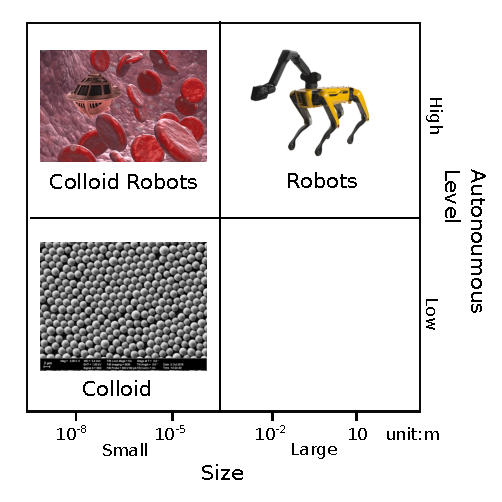
\includegraphics[width=9cm]{figures/1_1.pdf}
\caption{Colloid robots are a combination of the words "colloid" and "robots". Colloid robots are the same size as colloid particles from $\n m$ to$\mu m$ and usually suspend throughout the liquid phase. At the same colloid robots show dynamics autonomous behaviors such as motion, navigation, and communication, commonly seen in large robotics or living systems}
\label{fig:1.1}
\end{figure}


\section{Essential components for colloid robots}
Because colloid robots are still robots, the design for colloid robots can share some same basic principles and knowledge from large robotics systems.  Let’s look a typical robot system first. All of the robots have three essential parts actuators, sensors, and controllers. We would like to use cleaning robots as an example(as shown in figure1.2).  For cleaning robots,  there are two actuator systems. One is responsible for locomotion so that cleaning robots can move around in your apartment(wheels); the other actuation system is responsible for collecting and cleaning dirty spots on the floor(brush and squeegee vacuum).
The sensors for cleaning robots including infrared  sensors and cameras, which can sense the information in the environment. For example, the camera can help to see the location of dirty spots. The controllers are pre-programmed  to help cleaning robots plan  the actions. For example, if cleaning robots sense a corner, the controllers will let cleaning robots turn around to avoid crashing. One different thing about controllers is that controllers don't necessarily have physical parts. A controller can be a algorithm or a simple math function.  For all the robots, sensor , actuators, and controllers must work together as a feedback loop so robots can work functionally to finish different task: sensors collect information from the environment; based on information from sensors as well as the target of robots,  controllers will make decisions  on how to move actuators; then the actuators will drive robots into a new environment to repeating this feedback loop. This feedback loop composed of actuators, sensors,  and controllers is also the design guidance to build a colloid robot. However, due to size limitation and different physics regime of colloid robots, new mechanisms of actuation, sensing and controlling should be developed compared to the conventional approach in the large scale robots.  In the next section, we will address the challenge to build a colloid robot. 

\begin{figure}
\centering
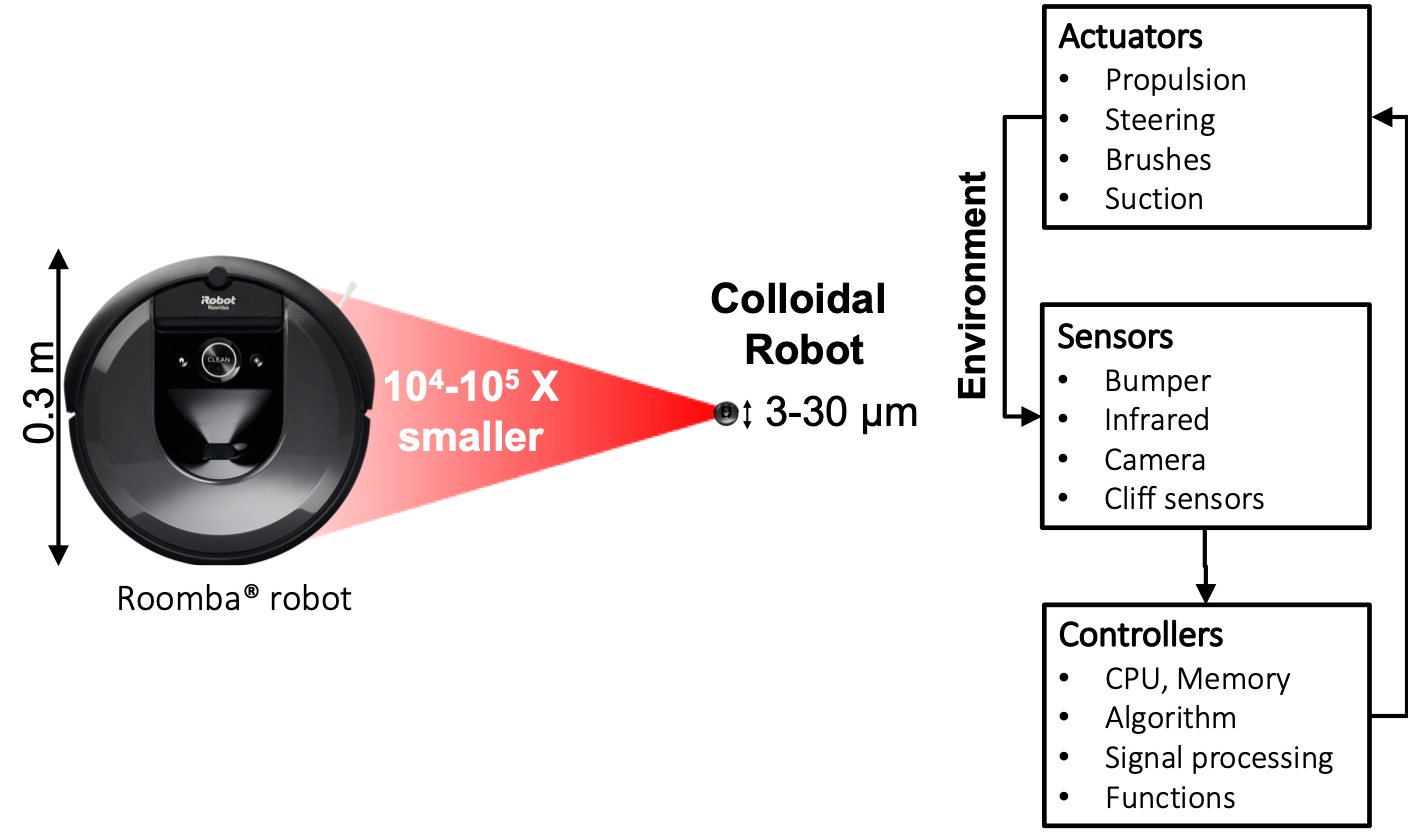
\includegraphics[width=12cm]{figures/1_2.png}
\caption{The essential components and feedback to design a colloid robot. In the feedback loop, sensors continuously collect information for controllers. Based on  information from sensors and targets of a robot, controllers will make decisions on how to drive the actuators.}
\label{fig:1.2}
\end{figure}

\section{The challenge to  build colloids robots}

\textbf{Size limitation}. In addition to the three basic components (sensors,actuators, and controllers) in the feedback loop, a robot also needs power supplies, manipulators with joints and a body frame, etc. Even for the simplest clean robot, there are around 100 parts inside. It is not possible to integrate all of these complex components in a micron-size particle(a micron size particle on a cleaning robot is just like a human standing on the earth)  if we simply follow the conventional method to build a normal size robot. 

\textbf{Physics limitation}. Physics for a colloid scale particle in the squishy  environment is very different from our normal size world, where everything becomes noisy and sticky. First, in the colloidal scale, Brownian motions largely affect the dynamics of colloidal particles, adding stochastic influence to the robotics. These thermal motions increase the difficulties in controlling the colloid robot's accuracy and precision. This requires the mechanism to drive colloid robots to be reliable enough to overcome the background noise. Second, the inertia totally disappears in the small scale as the Reynolds number of the colloid robot's system approach 0.  The Reynolds number presents the ration of inertia and viscosity represented as
\begin{equation}
    Re=\frac{\rho v l}{\mu}
\end{equation}
where $\rho $ is the density of fluid environment, v is the velocity of particle, l is the size of particle. $\mu$ is the  viscosity of fluid. In the colloid scale, both size and speed of particles are much smaller than 1, leading to the Reynolds number almost 0. The absence of inertia means all of the actuation method in normal size robots based on inertia will no longer work. This interesting  motion restriction in low Reynolds number is called Scallop
theory and was first discussed by Edward Purcell (Professor Prucell was famous for his independent discovery of something else(nuclear magnetic resonance, NMR), which brought him a Nobel prize) \cite{purcell1977life}. As shown in figure 1.3, Scallop Theorem states that a swimmer which exhibits time-symmetric motion cannot achieve net displacement in a low Reynolds number fluid environment because all the motion is time reversal. There is no difference between closing a scallop and opening a scallop. New actuation methods different large robot systems for colloid robots must be 

\begin{figure}
\centering
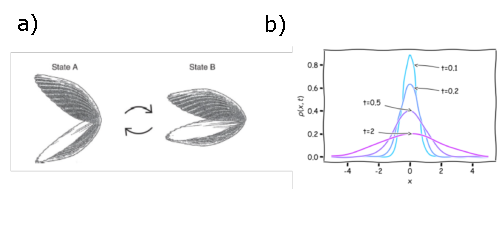
\includegraphics[width=8.5cm]{figures/1_3.pdf}
\caption{Physics challenge for building a colloid robot (a) Scallop theory. In the colloid scale, the effect of inertia almost disappears, making everything time reversal. (b) Brownian motion. The presence of thermal noise in the colloid scale let the motion of colloid robots unpredictable.}
\label{fig:1.3}
\end{figure}
To solve the  challenges mentioned above and design the colloid robots, researchers got inspired from real small living  machines. The dynamic functions of living cells require integration of structures and processes to drive material organization in space and time. For example in the muscle cell,  the coupling of complex structures(kinesin motor protein) and dissipative processes (ATP hydrolysis) can generate mechanical work.(see fig 1.4) Thus, a colloid robot should also have both complex structures and a dissipative process. Thanks to the development of nano/micro scale fabrication in the semiconductor industry, we can now create materials with heterogeneous structure and composition on length scales spanning molecular to macroscopic dimensions with chemical synthesis, lithography, deposition , and etching. These technologies can be directly transplanted to the fabrication process of colloidal robots. In addition to structural and material complexity, the artificial dissipation process(or actuation process) for colloid robots  can be generated  with chemical reaction, external field(electric, magnetic, acoustic or fluid flow) to generate motion breaking the time reversal constraint. For the past decade, lots of research has been conducted to engineeringly build colloid robots  or study the fundamentals of colloid robots. The Colloid robot is now a emerging interdisciplinary field attracting many scientists with different background from math, physics to chemistry, biology and engineering. A state-of-art  review on colloid robots' research is going to be reviewed in the next section.
\begin{figure}
\centering
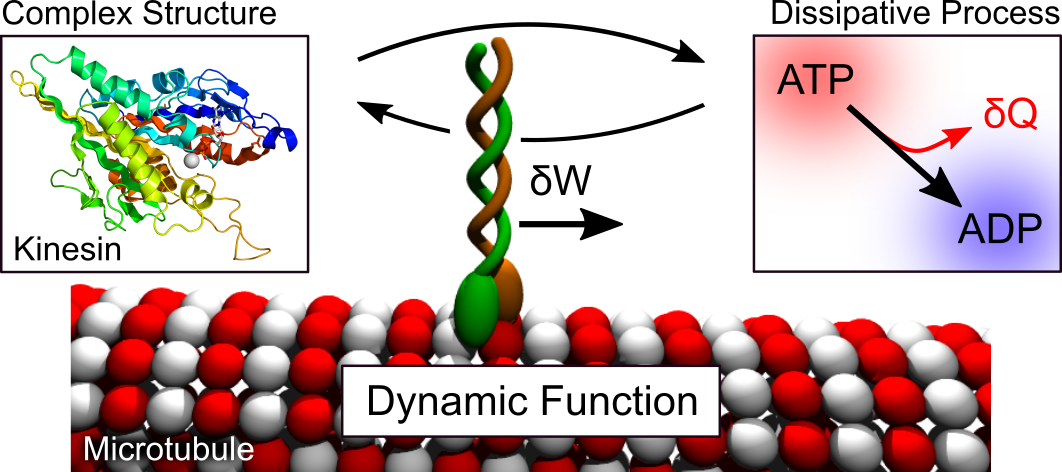
\includegraphics[width=8.5cm]{figures/1_4.png}
\caption{Dynamic functions require the coupling of complex structures and dissipative processes–here, a kinesin motor protein bound to a microtubule  does work powered by ATP hydrolysis}
\label{fig:1.4}
\end{figure}

\section{A state of art review on colloid robots }
It is not clear which paper first mentioned the similar idea of colloid scale robotics(the original concept of  small scale machines can be tracked to Richard Feynman's famous paper,\textit{There's plenty of room at the bottom}\cite{feynman1960there}). The current research wave in the past decade on the colloid robots is triggered by the discovery of self propulsion active colloid particles driven by chemical fuels \cite{paxton2004catalytic}. In 2004, scientists from Penn State University found that chemical fuel(they use hydrogen peroxide, $H_2O_2$,  in their first paper) can drive  gold-platinum bimetallic nanorods' autonomous motion. The asymmetric different chemical reactions, which happen at the different end of their nanorod,  lead to a net flow fluid near the surface of nanorod. This pioneer research then attracted lots of attention in different research field beyond chemistry such as soft condensed matter physics\cite{Marchetti2013}, materials science\cite{han2018engineering}, applied math\cite{fodor2016far} and engineering \cite{sitti2015biomedical}. More than tens of thousands of papers related to the autonomous behaviors of colloids have been published since then. However, most of these research papers either experiment or theory only focus on building actuators for colloid robots. Only a few of them realize some complex tasks with colloid robots such as navigation. From our knowledge, the higher level's automation is still challenging, and should be the main research direction in the future. In the following content, we are going to give a short state-of-art review on both experiment approach to colloid robots as well as some basic theories and simulation methods for colloid robots. In this short review, we have no intention and interest to rephrase and cover all the research papers on colloid robots like an encyclopedia book. Instead,  I will focus on the main physics, chemistry and engineering ideas behind these papers. 

\subsection{Experiment approach}

\textbf{Fabrication}  High throughput nano/micro scale fabrication technologies in semiconductor manufacturing industry now can make a 3-D structure even smaller than 5$nm$.\cite{mokhlesi2010three} These fancy technologies to make CPU and memory in electronic devices can be transplanted directly to make colloid robots with almost any desired size, shape and component in cleanroom.\cite{koman2018colloidal} A typical fabrication process mainly including lithography to make patterns as the main body and frame for colloid robots , etching to remove unnecessary materials and deposition to introduce new materials. Multi-layer processing can be designed and optimized to make high dimensions and complex structure such as spiral shape\cite{zhang2009artificial}. After the colloid robots are fabricated on the wafer, they can be harvested from the silica surface with etching technology or simply physical removal. For the detailed process of fabrication, I would like to refer readers to these three comprehensive reviews\cite{wong2016synthetic,wang2017emerging, zha2018tubular}. Chemists and material scientists also contributed creative chemical synthesis methods to make colloid scale complex structure with one-pot high-throughput method\cite{youssef2016shape,gong2017patchy,wang2019active}. One challenge for colloid robots' fabrication is to   make  colloid scale soft(or shape-shifting) structures with complex components. Liquid crystal, hydrogel gel, droplet, silica polymer and self-assembled nanoparticles are promising candidate materials for micro/nano scale soft structure. \cite{leong2009tetherless,denkov2015self,zhang2017printing,wei2019molecular}. Another fabrication challenge is to make bio-hybrid colloid robots which can take advantage of  properties in real living systems. Bio-hybrid colloid robots require high compatibility  among different materials, where experimental biologists can provide invaluable experience and knowledge.\cite{stanton2016biohybrid,magdanz2013development}

\textbf{Actuation} Autonomous motion is the most basic characteristic of colloid robots, making colloid robots real machines instead of simple colloid particles. Colloid robots can harness energy from the environment and convert energy into mechanical work. Compared to the inertia driven mechanism in normal size robot, the actuation of colloid robots always experiencing large hydrodynamics resistance force to balance the driving force. The actuation's power source can be divided into two main categories: chemical/biochemical reactions and the external physical fields. Living cells and bacteria use a series of  chemical reaction networks (e.g. ATP hydrolysis) to convert their food source to motions. Colloid robots can also mimic this life-like energy conversion mechanism by implementing the chemical reactions on the surface of colloid particles. The reactions happen between the material of colloid robots and chemical species in the fluid environment. Colloid robots can work as a catalyst or reactant to trigger the reaction in the fluid environment. For example,  colloid robots can be made of gold or metal,  which catalysis the hydrogen peroxide in the fluid to water and oxygen. During the fabrication process, these catalysis or reactant material are patterned at different places of colloid robots to break the symmetry generating chemical species' gradient or reaction product(e.g. bubbles) to actuate colloid particles \cite{velegol2016origins,shklyaev2016harnessing,parmar2018micro}. Recent reports also showed biochemical reaction(e.g. enzyme) can be options to drive colloid robot's motions, although the mechanism is still controversial.\cite{zhao2018substrate,somasundar2019positive}

In addition to  chemical reactions, almost all the external physical field have been used to powering autonomous motion of colloid robots including electric\cite{lee2019directed}, magnetic\cite{zhang2009artificial}, acoustic\cite{sabrina2018shape}, light\cite{dai2016programmable}, or thermal field\cite{lozano2016phototaxis}.  Colloid robots programmed with physical monopole, dipole or quadrupole will respond to the external physical fields, leading to rotational or transitional motion. For example, colloid robots can be fabricated with magnetic materials such as nickel and cobalt to a have magnetic dipole moment. Then an external magnetic can generate a torque on the colloid's magnetic moment, manipulating the autonomous motion. Compared to the  chemical reaction actuation method, an external physical field can drive colloid robots' motion with less fluctuation. \cite{han2018engineering,ren2018two}. 
The current biggest issue in actuation of colloid robots is the very low energy efficiency(usually in the order magnitude of $<10^{-5}$ or less). Colloid robots always dissipate large amounts of heat\cite{wang2013understanding} compared to the real living cells which can perform efficient motion with much less heat dissipation.

\textbf{Coupled actuation}  In addition to a single colloid particle's actuation,  colloid robots can also be actuated via many actuators' interaction and coupling similar to the multi-cylinder engine in a car. These coupled actuation behaviors can perform some life-like collective functions seen in birds' swarm and fish's flock \cite{wang2015one,ginot2018aggregation}. Emergent patterns, dynamic clustering, and phase separation have been observed  in different colloid robot systems. \cite{buttinoni2013dynamical,ginot2018aggregation,duan2013transition,theurkauff2012dynamic} The interactions among colloid robots are usually in two forms. One is pure force interaction with each other. For example charged colloid robots have electrostatics interactions. \cite{dou2018emergence} The second kind of interaction is indirect influence. One colloid robot's motion and dynamics  will have an influence on the fluid environment, then  the fluid environment will exert this influence back to other colloid robots in the same environment. Most of the second type interactions are hydrodynamic or chemical reactions. For example, the hydrodynamics flow induced by one colloid robots will attract/repel other colloid robots from it. \cite{karani2019tuning} Although colloid robots showing collective behaviors can interact with each other, this kind of communication and interaction is passive and lack of programming. Colloid robots cannot take pre-programmed actions from controllers for some desired tasks when they are exerted on some interactions--most papers studying collective behaviors of colloid robots only observe the phenomena instead of  programming the dynamics.  As a comparison, in normal size robots research, distributed robotics or  swarms robotics\cite{wei2010sambot,arvin2014colias} can also show life-like dynamics behaviors, but they are more intelligent. These robots can communicate with the electronic signal instead of pure physics force. They can not only interact with each other, but also perform programmed reactions and different tasks.\cite{rubenstein2012kilobot,rubenstein2014programmable,li2019particle}

\textbf{Navigation} All the living cells or batteries can sense the information from the environment to navigate themselves for energy, food, or suitable living place called \textit{taxis} behaviors. Autonomous colloid robots should capable of the same kind of navigation abilities. Not so many experiments approach haven been showed to demonstrate  artificial taxis in colloid robots compared the large amounts of papers on simply showing autonomous motions. Current approaches mainly belong to two mechanisms: computational vision feedback system and physical force "correction" method. The computational vision feedback system uses a microscope with digital camera to track the location and velocity of colloid robots online with a computer vision algorithm. Then based on the information of location, speed of colloid particles, and the desired navigation direction, the computer(controllers) will compute the proper external field that should be applied in the next time point. The "tracking-computing-applying new field" feedback loop will continue until colloid robots reach the destination\cite{li2017autonomous,han2017sequence} This method has several big defects. The first disadvantage is the size of the whole system. The navigation behaviors have to be coupled with complex external devices(microscope, camera, computer) which is not portable and convenient. Second, this mechanism cannot apply to a large number of colloid robots with different location and velocity because the external physical field can only satisfy one particle's navigation requirement. The physical force "correction" method can navigate  colloid to transport following  some gradient information mimicking a living taxis behavior. This method uses the local gradient information(e.g.light intensity, chemical species concentration, temperature) or asymmetric geometry to generate torque rotating  the colloid robot to "correct" its orientation aligning with the gradient. Then the colloid robot can move along with gradient in the environment showing navigation behaviors \cite{brosseau2019relating,ten2014gravitaxis,lozano2016phototaxis,baker2019fight} However the physical force correction method  lacks the robotic feedback with controller and sensors. With this mechanism, a colloid particle can only be navigated into one direction, which can't be easily re-programmed for doing other types of navigation tasks in a different environments. All of the problems for the current approach to autonomous navigation mentioned above is due to the lack of sensors and controllers in the colloid scale for colloid robots





\subsection{Theory and simulation}
Richard Feynman said "What I cannot create, I do not understand." to emphasize the importance of fundamental understanding of science. This is also true for the  research in colloid robots. To design a colloid robot of higher automation level, understanding the physics and mathematics behind it is as  important as  experimental attempts. Colloid robots are operated far from the equilibrium state with constant energy and mass flow. Recently years there has been intensively research on non-equilibrium matter, called active matter, in the community of soft matter and statistic physics. Some study is focusing on building a generally high-level theoretical physics framework for active matter with continuum mechanics or statistical mechanism. \cite{stenhammar2013continuum,solon2015pressure,fodor2016far}. Lots of papers are also trying to use simulation or toy models to discover and design new dynamics behaviors in colloid robots. \cite{bechinger2016active,speck2014effective,ten2011brownian}. In this section,  basic physical features and mathematical descriptions are going to be reviewed for colloid robots.  Deeper and detailed derivation can be referred to our citations.

\textbf{Brownian motion} Colloid robots' motion is influenced by the thermal noise(Brownian motion) in the fluid environment because of their small size. The Brownian motion can be described with Einstein–Smoluchowski Diffusion Equation.\cite{islam2004einstein} If we take the colloid robot as  a rigid spherical body, the translation and rotation diffusion coefficients are: 

\begin{equation}
    D_T=\frac{k_B T}{6 \pi \eta R }
\end{equation}
\begin{equation}
    D_R=\frac{k_B T}{6 \pi \eta R^3 }
\end{equation}
where $k_B$ is the Boltzmann constant, $T$ is temperature of the environment, and $\eta$ is the viscosity of fluid, $R$ is the radius of colloid robots. The diffusion characteristic time is the 
reciprocal of diffusion coefficient, as  $\tau=D^{-1}$. As the size of colloid robots decrease, the rational diffusion coefficients$D_T$ increase much faster than transnational diffusion coefficients$D_R$. For an actuated colloid with autonomous motion velocity as $v$ in two dimensions, the dynamics can be described as,
\begin{equation}
    \frac{dx}{dt}=v Cos(\theta)+\sqrt{2 D_T}\xi_x, \quad \frac{dy}{dt}=v Sin(\theta)+\sqrt{2 D_T}\xi_y,\quad
    \frac{\theta}{dt}=\sqrt{2 D_R}\xi_\theta
\end{equation}
Where $\xi$ is the independent noise with mean as $0$ and correlation as $\delta(t)$. In chemical engineering, we use the Péclet number to represent the dimensionless ratio between convection  and diffusion. For colloid robots, the Péclet is 
\begin{equation}
    Pe\propto\frac{v}{\sqrt{D_T D_R}}
\end{equation}
to characterize the influence of Brownian motion on the actuated autonomous motion.

\textbf{Actuated force} As introduced in the previous section, actuation mechanisms are divided into chemical reactions and physical field actuation. For the chemical reactions driven colloid robots, the phoretic interaction  model describes the system very well. \cite{golestanian2007,najafi2004simple,golestanian2005propulsion,golestanian2019phoretic} In this model, the reaction rates are considered much faster than the diffusion rate of chemical species, resulting in the following   
quasi-stationary reaction-diffusion equation,
\begin{equation}
    -D\nabla^2 C=0
\end{equation}
where D is the diffusion coefficient of reactant, this is the Laplace equation for concentration in the fluid environment. The boundary condition for this Laplace equation is  colloid robots' consuming or producing chemical species as,
\begin{equation}
    -D \texbf{n}\cdot \nabla C|_{r=r_s}=\alpha(r_s)
\end{equation}
where $r$ is the distance from the center of colloid, $r_s$ is the radius of colloid, \texbf{n} is the normal vector on the surface of colloid and $\alpha(r_s)$ is the flux rate. The chemical reaction will lead to a net normal flux(denoted as $\alpha(r_s)$ ) on the surface of colloid. The fluid will response to the local gradient change near the colloids and generate a slip velocity as,
\begin{equation}
    v_s=\mu(r_s)(\textbf{I}-\textbf{n}\textbf{n})\cdot \nabla C(r_s)
\end{equation}
$\mu$ is called mobility measuring the response rate of fluid to the concentration gradient. By making $\alpha$ and $\mu$ positive or negative, the asymmetric chemical activity on the surface can lead to autonomous motion.  Also, both repulsion and attraction forces between colloids can be achieved to study collective behaviors of this system. \cite{michelin2015autophoretic}

For the external physical field actuation, the force exerted on each component colloid robot following the corresponding law of physics. For example, charged colloid robots with charge amount $q$ experienced electrostatic force $Eq$ in the electric field $E$; magnetic colloid with dipole $m$ in a magnetic field $B$ can be actuated with torque $m\times B$.
Then we can calculate the total force and torque on the rigid body colloid robots via doing the surface integration if the force is exerted on the surface.
\begin{equation}
    F=\oint_S f_e \,dS
\end{equation}
\begin{equation}
    T=\oint_S (x-x_c)\times f_e \,dS
\end{equation}
Where $f_e$  is the component of the actuated force and $x_c$ is the center of colloid robots.

\textbf{Hydrodynamics}  The in-compressible viscous fluids are governed by Navier–Stokes equations without any inertia component as discussed in the previous section,
\begin{equation}
    \eta \nabla^2\textbf{u}-\nabla p=0,\quad \nabla \cdot u=0
\end{equation}
where $\eta$ is the viscosity, p is the pressure from fluid. Although hydrodynamic problems are the most complex ones in modeling colloid robots because of non-linear terms, it is also the most interesting modeling research part with lost of  nontrivial and unexpected results and patterns. \cite{Lauga2009,berke2008hydrodynamic,lauga2011life} In the low Reynolds number regime, the hydrodynamic force will balance the external force generated by the actuation mechanism. Stokesian dynamics are used to calculate the  translation and angular velocity of colloid robots \cite{Brady1988a,Kim2005}
\begin{equation}
    \left[ \begin{array}{c} F \\ T \end{array} \right] = \begin{bmatrix} A & B \\ B^T & C \end{bmatrix} \left[ \begin{array}{c} v \\ \omega \end{array} \right]
\end{equation}
where \textbf{A}, \textbf{B}, and \textbf{C} are tensors determined only by the shape and orientation of the colloid robots. The whole big matrix is called resistance tensor, which can be calculated analytically\cite{Kim2005}  Tensor \textbf{B} is called coupling tensor to couple the transition and rotation together. Resistance tensor is no longer symmetric if boundary exists in the fluid environment.  Stokesian dynamics  can be extended to calculate the hydrodynamics interactions between each other via Faxen's law.
\begin{equation}
    F_{drag}=6 \pi \eta a((1+\frac{a^2}{6}\nabla^2)v_{\infty}(0)-U)
\end{equation}
Where $F$ is the   force exerted by the fluid on the colloid particles, $a$ is the size of colloid, $u$ is the  the translation  velocity of the colloid and $v$ is the disturbance velocity caused by the presence of other colloids in the fluid environment. We would rather direct our readers to James Swan's paper for the full expression of hydrodynamic interaction in the form of Stokesian dynamics. \cite{swan2011modeling} Basically, the simulation of colloid robots' dynamics are solving partial differential equations either numerically or analytically with the physical model showed above. In addition to some commercial multiphysics simulation software such as COMSOL\textregistered, there are also some open-access library written in various coding languages  can help to simulate the dynamics of colloid robots. \cite{glaser2015strong,anderson2008general,swan2011modeling,singh2019hydrodynamic}

\textbf{Design and optimization} For engineering purposes, colloid robots should be designed with desired functions.\cite{liebchen2019optimal} As shown in figure 1.6 the design process should start with constructing and understanding the design parameters space. For example how many physics variables(e.g size, temperature, fluid viscosity, choice of materials) should be added into our design space. And then we  need to reduce the dimension of the design space based on physics and mathematics to make then design problems easier. Dimension reduction is a very essential part of the colloid robot's design problem. A good dimension reduction will significantly reduce the time searching for the optimized result. Then we build a physical model to link these design parameters and our target functions of colloid robots together. This physical model should be adequate enough  to capture call the key physics affecting the dynamics of colloid robots. At the same time, this model should be concise enough to eliminate unnecessary computation work. After the forward modeling is constructed, we can reverse design the parameter of colloid robots by defining the desired performance functions such as the highest velocity, lowest efficiency. Then the final step is to use an optimization algorithm to find the optimal parameters in the design space for the reverse problems. \cite{ward1963hierarchical,nocedal2006numerical} Recent research also shows that machine learning technology can assist to design colloid robots with impressive efficiency .\cite{yang2020micro,yang2020cargo,yang2019deep,tsang2018self}
\begin{figure}
\centering
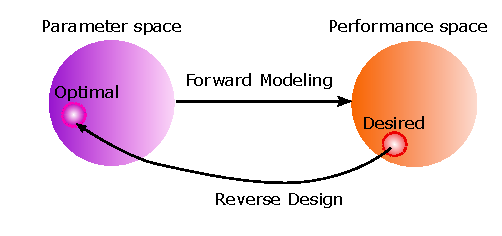
\includegraphics[width=8.5cm]{figures/1_6.pdf}
\caption{The forward modeling connects the design space and performance of colloid robots together. With the reverse design, the optimal parameters to build a colloid robot with the desired function can be found.}
\label{fig:1.6}
\end{figure}


%\textbf{Potential Application }
